\فصل{روش $Knuth-Yao$}

در این الگوریتم از یک درخت به نام درخت تولید اعداد گسسته  $discrete distribution generating (DDG)$   استفاده می کنیم . 
اگر  بخواهیم تعدادی اعداد  تصادفی داشته باشیم با بردار احتمال $p_{1}, p_{2}, ...$ -که می تواند محدود یا نامحدود باشد- داشته باشیم، می توان هر کدام از این احتمالات را به صورت رشته دودویی نوشت و از روی آن یک درخت ساخت که بیت‌های این رشته را نمایش می دهد. این درخت دو نوع گره میانی و انتهایی دارد . با حرکت تصادفی بر روی این درخت می توان عدد تصادفی را انتخاب کرد. 
 گره های میانی : این گره‌ها دو فرزند دارند . هنگامی که بیت جاری صفر باشد به فرزند سمت چپ می رویم و هنگامی که بیت جاری یک باشد به فرزند دوم می‌رویم. 
 گره های انتهایی : این گره‌ها فرزندی ندارند . این گره‌ها با یک عدد صحیح  که در واقع همان عدد تصادفی مورد نظر ما هستند ، مشخص شده اند که این عدد را برمی‌گردانند.(devroy)

      \begin{figure}[!htb]
      	\minipage{1\textwidth}
      	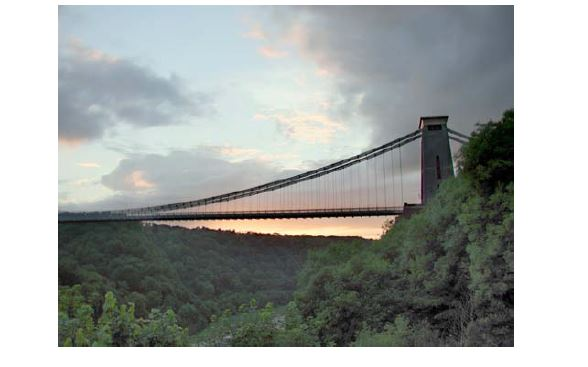
\includegraphics[width=\linewidth]{images/retinex1}
      	\caption{retinex}\label{fig:logtonemap}
      	\endminipage\hfill
      	% 	\centerline{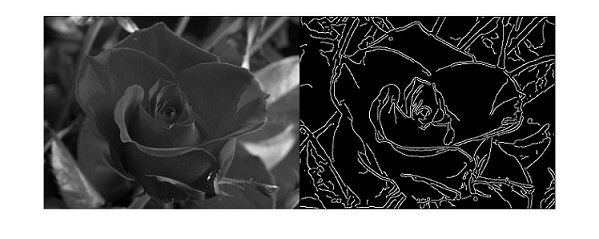
\includegraphics{images/cannyexample2}}
      \end{figure}
      
روش $Knuth-Yao$ برای نمونه برداری از توزیع غیر یکنواخت مناسب است . فرض کنید که فضای نمونه از$ n$  عنصر $0\< r \< n$با احتمالات  $p_{r}$ ساخته شده است . این احتمالات را همان طور که در بالا گفته شد، به صورت اعداد دودویی در می آوریم.   با استفاده از این احتمالات یک ماتریس احتمال می سازیم و اسم آن را $P_{mat}$  می‌گذاریم . سطر $ r$ ام این ماتریس احتمال عدد$ r $ام را که به صورت دودویی نوشته شده است را  نمایش می دهد. که در هر ستون یک عدد دودویی قرار می دهیم .  در مثال ذکر شده در شکل .... می خواهیم از میان سه عدد 0و1و2  یک عدد را با توجه به احتمال آن به طور تصادفی انتخاب کنیم . احتمال به صورت $p_{0}= 0.01110, p_{1} = 0.01101, p_{2} = 0.00101$ است. 
درخت $DDG $را  بر اساس ماتریس احتمالات ساخته می‌شود. در هرعمق از درخت می توان  هر یک از دو نوع گره - گره میانی $(I)$ و گره انتهایی - را داشته باشیم . تعداد گره‌های انتهایی در سطح $i$ ام برابر است با وزن همینگ ستون $i$ ام از ماتریس احتمال $P_{mat}$.  در مثال ذکر شده ریشه دو فرزند دارد که سطح صفر را تشکیل می دهد. به دلیل آنکه وزن همینگ ستون صفر ماتریس $P_{mat}$ برابر صفر است و هیچ عدد غیر صفر ندارد؛ هر دو این گره، گره میانی    $(I)$  هستند . این دو گره میانی چهار فرزند در سطح یک دارند. برای اینکه نوع گره‌ها مشخص شود اولین ستون ماتریس $P_{mat}$ از سطر آخر بررسی می شود. در این ستون تنها سطر یک و صفر اعداد غیر صفر دارند ، بنابراین  دو تا سمت راست‌ترین گره‌ها در سطح یک درخت به ترتیب  1 و 0 برچسب می‌خورند. دو گره باقی‌مانده هم به عنوان گره‌های میانی برچسب گذاری می‌شود. به طور مشابه سطح بعدی هم ساخته می شود. درخت ساخته شده از ماتریس مثال در شکل .... نشان داده شده‌است.در هر سطح درخت $DDG$ در صورت وجود گره انتهایی، این گره‌ها همیشه در راست‌ترین سمت درخت قرار می‌گیرند.
 نمونه برداری بر اساس راه رفتن تصادفی برروی درخت انجام می شود . با توجه به ورودی تصادفی  می توان در هر قدم به فرزند راست یا به فرزند چپ رفت . این الگوریتم زمانی پایان می پذیرد که در راه رفتن تصادفی به یک گره انتهایی برسیم و خروجی الگوریتم همان مقدار آن گره انتهایی است. جرکت تصادفی $Knuth-Yao$ از توزیعی که توسط ماتریس احتمال معرفی شده است ، از اعداد نمونه‌برداری می‌کند.
درخت $DDG$ به اندازه $O(nk)$ حافظ  نیاز دارد که $k $ تعداد ستون‌های ماتریس احتمال است . می‌توان با ساخت درخت $DDG$ در زمان اجرا فضای مورد نیاز را کمتر کرد و در هر مرحله تنها یک سطح را نگه داشت . در حقیقت سطح $i $ام   درخت $DDG$ از روی سطح $i-1$   ام درخت و ستون $i$ ام ماتریس احتمال ساخته می شود . بهینه تر است که تنها اطلاعات یک عمق را نگه داریم و عمق بعدی را از روی آن بسازیم. 
ساخت درخت DDG  هنگام نمونه برداری: 



در هنگام راه رفتن تصادفی در روش $Knuth-Yao$ درخت $DDG $ در زمان اجرا ساخته می‌شود. همان‌طور که قبلا گفته شد استفاده از درخت DDG  تنها نیازمند آن است که اطلاعات یک سطح قبل را نگه داری کنیم . سطح$ i$ ام حداکثر$2^{i}$ تا گره دارد$(2^{i} \< nk)$  . در درختهای$ DDG$ تمام گره‌های میانی در سمت چپ درخت قرار دارند و تمام گره‌های پایانی در سمت راست قرار دارد.  شکل ... سطح $ i - 1$  را نشان می‌دهد. در این شکل گره‌های میانی $I$  و گره‌های انتهایی $T$  می‌باشند. گره‌ای که در این سطح بررسی می‌شود توسط دایره دوتایی مشخص شده‌است. فرض میکنیم که گره‌ای که در این مرحله  بررسی می‌شود گره انتهایی نیست چرا که می خواهیم عمق بعدی را بسازیم.بنابراین این گره یک گره $I$ می‌باشد. فرض می‌کنیم که در عمق $i - 1$  ،  به تعداد $n $ گره میانی وجود دارد و گره جاری $k$  امین گره از سمت چپ است . بنابراین $d= n - k$ تعداد گره میانی از گره جاری تا گره‌های انتهایی عمق $i - 1$ وجود دارد . حال با توجه به ورودی تصادفی به فرزند چپ یا راست می رویم . اگر فرزند چپ انتخاب شد به تعداد $2d + 1$ گره در سمت راست آن وجود دارد در غیر این صورت در زمانی که فرزند راست انتخاب شد تعداد $2d$  گره در سمت راست خود دارد (شکل ...) . برای این‌که مشخص شود گره فرزند دیده شده یک گره میانی است یا انتهایی به ستون $i $ام ماتریس احتمال توجه می‌کنیم . وزن همینگ را در ستون $i$  ام برابر $h$  می‌گیریم . اگر این فرزند ، فرزند چب باشد اگر h > 2d+ 1 آنگاه این فرزند یک گره انتهایی است و اگر   فرزند، فرزند راست باشد آنگاه اگر h > 2d  انگاه فرزند یک گره انتهایی می شود که مقدار آن برابر است با  سطر مربوطه ..... . اگر گره دیده شده یک گره میانی باشد دوباره سطر i + 1  از روی سطر i  ام  ساخته می شود . 
با تحلیل درخت DDG  می توان نکته های زیر بیان کرد :
1- نمونه برداری مستقل از گره های داخلی است  که در سمت چپ گره دیده شده هستند. 
2- گره انتهایی که در عمق i - 1  قرار دارد هیج تاثیری در ساخت عمق i  ام ندارد. 
3- فاصله d - فاصله گره جاری دیده شده تا گره های انتهایی همان عمق-   برای این که مشخص شود که گره دیده شده در عمق i  ام  یک گره انتهایی است یا میانی ، کافی می باشد. 
الگوریتم knuth-Yao  در الگوریتم .... نوشته شده است. همان طور که دیده می شود در خط 6  عدد تصادفی r برای پرش به عمق  بعدی و اینکه فرزند راست یا چپ انتخاب شود ، درست می شود. با توجه به اینکه عدد تصادفی r  چه باشد فاصله فرزند دیده شده تا راستترین گره 2d یا 2d + 1  می شود .در خط 8 for-loop  یک ستون را برای اینکه گره انتهایی را پیدا کند ،  چک می کند. هر زمان که الگوریتم یک ، 1 پیدا کرد ، یک گره پایانی پیدا کرده است   ................... هنگامی که d  به -1 می رسد ، الگوریتم نمونه برداری .....
کم کردن اندازه ماتریس Knuth-Yao
  
  
  
  \begin{figure}[!htb]
  	\minipage{0.48\textwidth}
  	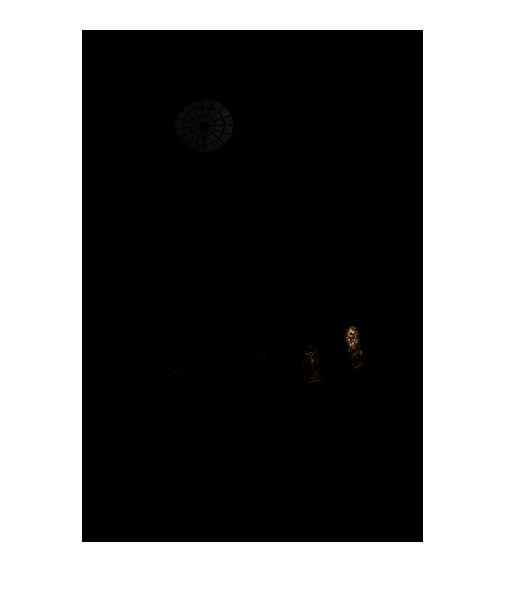
\includegraphics[width=\linewidth]{images/linearhdr1}
  	\caption{linear}\label{fig:logtonemap}
  	\endminipage\hfill
  	\minipage{0.48\textwidth}
  	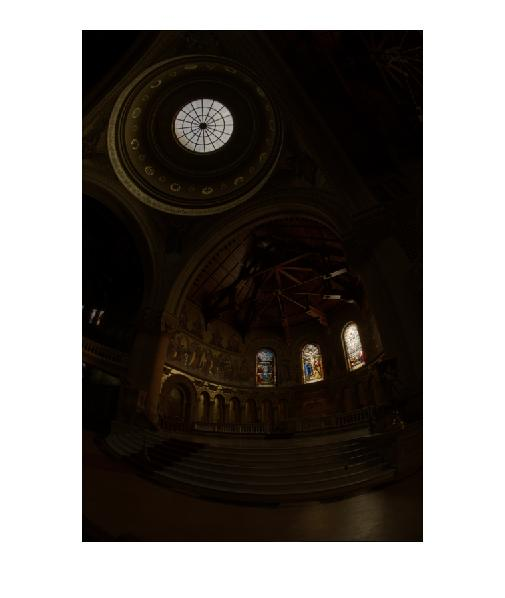
\includegraphics[width=\linewidth]{images/loghdr1}
  	\caption{logarithmic}\label{fig:lineartonemap}
  	\endminipage\hfill
  	% 	\centerline{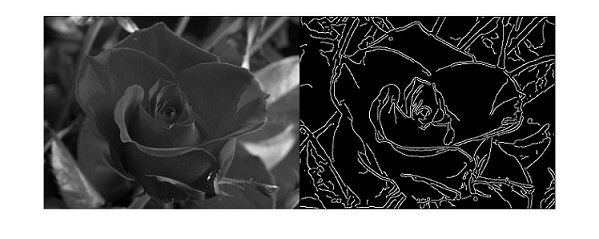
\includegraphics{images/cannyexample2}}
   \end{figure}
      
  \begin{figure}[!htb]
    \minipage{1\textwidth}
      	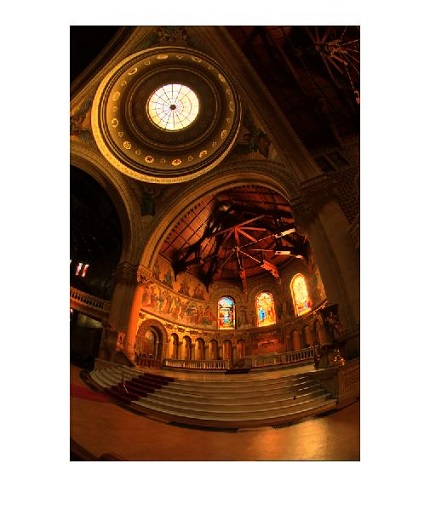
\includegraphics[width=\linewidth]{images/reinhardhdr1}
      	\caption{rainhard}\label{fig:logtonemap}
    \endminipage\hfill
      	% 	\centerline{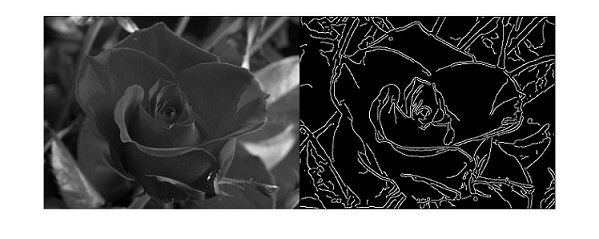
\includegraphics{images/cannyexample2}}
   \end{figure}
      
        
    \begin{figure}[!htb]
     \minipage{1\textwidth}
        	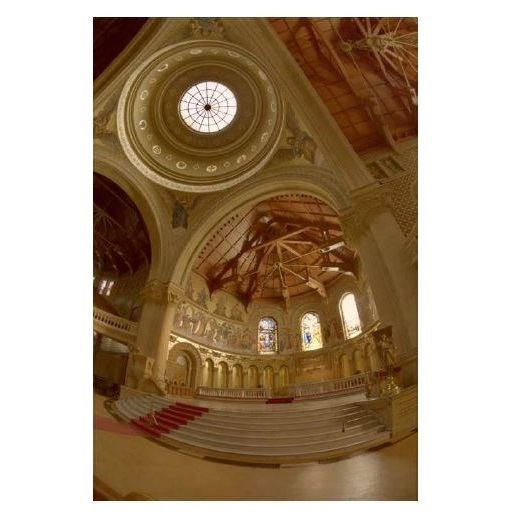
\includegraphics[width=\linewidth]{images/retinex3}
        	\caption{retinex}\label{fig:logtonemap}
      \endminipage\hfill
        	% 	\centerline{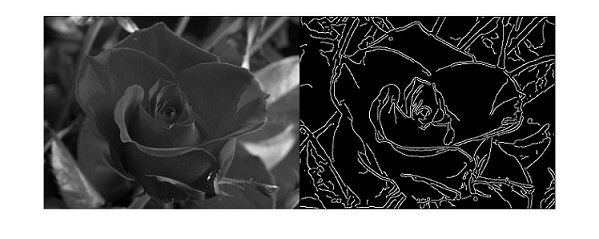
\includegraphics{images/cannyexample2}}
    \end{figure}
        
        
      \begin{figure}[!htb]
      	\minipage{0.48\textwidth}
      	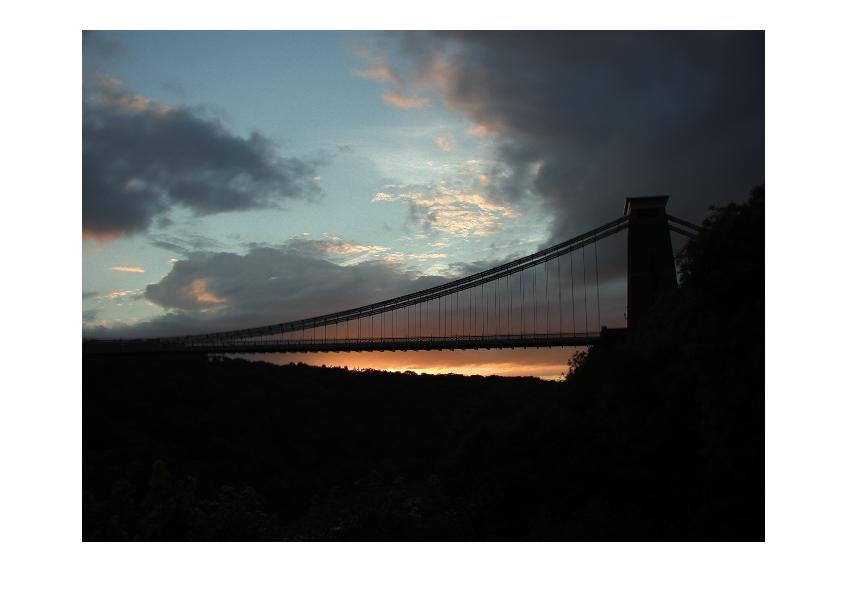
\includegraphics[width=\linewidth]{images/linearhdr3}
      	\caption{linear}\label{fig:logtonemap}
      	\endminipage\hfill
      	\minipage{0.48\textwidth}
      	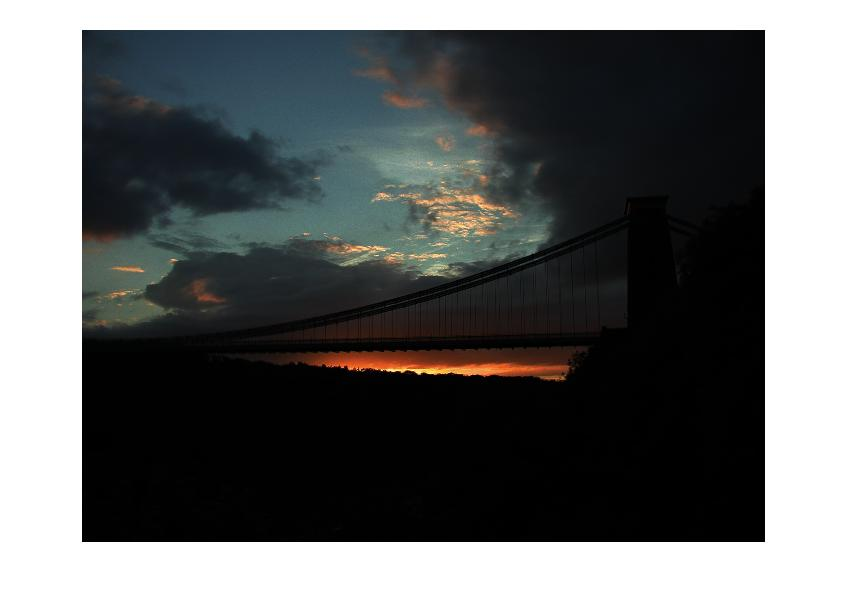
\includegraphics[width=\linewidth]{images/loghdr3}
      	\caption{logarithmic}\label{fig:lineartonemap}
      	\endminipage\hfill
      	% 	\centerline{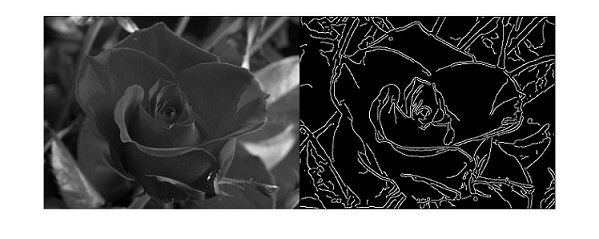
\includegraphics{images/cannyexample2}}
      \end{figure}
      
      \begin{figure}[!htb]
      	\minipage{1\textwidth}
      	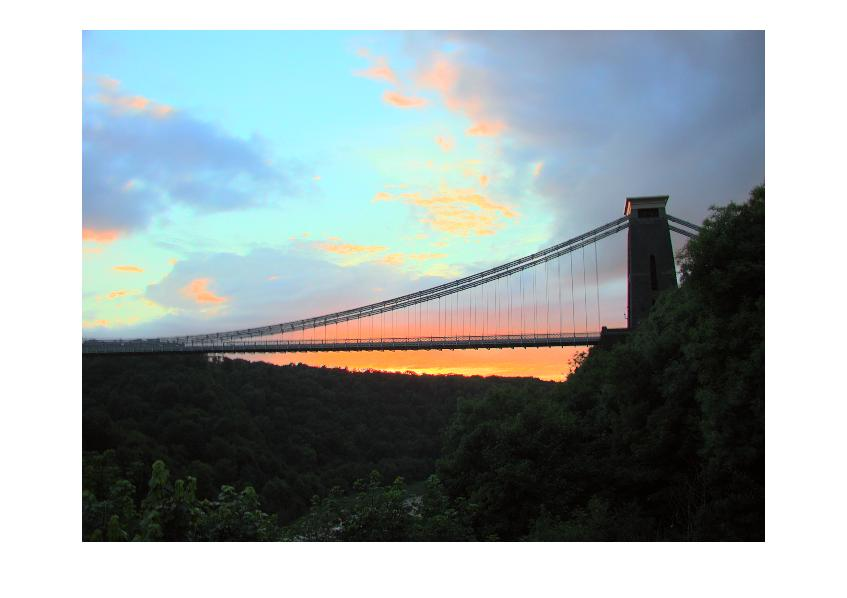
\includegraphics[width=\linewidth]{images/rainhardhdr3}
      	\caption{rainhard }\label{fig:logtonemap}
      	\endminipage\hfill
      	% 	\centerline{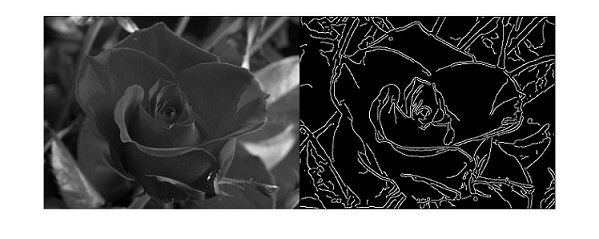
\includegraphics{images/cannyexample2}}
      \end{figure}
      
      
      \begin{figure}[!htb]
      	\minipage{1\textwidth}
      	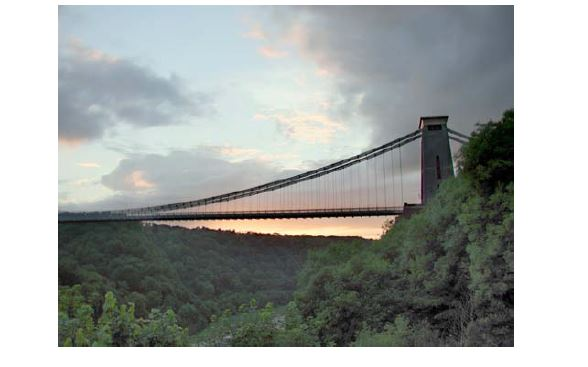
\includegraphics[width=\linewidth]{images/retinex1}
      	\caption{retinex}\label{fig:logtonemap}
      	\endminipage\hfill
      	% 	\centerline{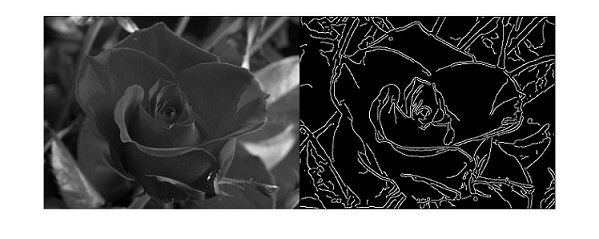
\includegraphics{images/cannyexample2}}
      \end{figure}
         